\chapter{Fine-tuning Enhanced ASR}
\label{chap:fine_tune_enhanced}
In \cref{chap:enhanced_asr}, we proposed the ``Enhanced ASR'' pipeline (see \cref{fig:asr_enhanced_pipeline}) which consists of an \emph{acoustic} model and a \emph{phoneme-to-grapheme translation} model. So far, we used ``clean'' (without any errors) training data to train the translation model. The obvious problem is that the phoneme transcripts produced by the acoustic model in the ASR pipeline will most probably contain errors, to which the translation model is not ready.

In this chapter, we review the fine-tuning of the ASR translation model to errors introduced by the acoustic model.

This chapter is organized as follows: in \cref{feasr:related} we review the related work. \cref{sec:asr_corrupted,sec:asr_corrupted_cs} describe process in which we obtain training data with ``ASR errors''. Finally, \cref{easr:easr} reviews setups for final part of proposer Enhanced ASR pipeline and trains it.

\section{Related Work}
\label{feasr:related}

\citet{hrinchuk2019correction} deal with the correction of errors in ASR by introducing a Transformer post-processing step. 

The authors first train an ensemble of 10 Jasper ASR models on the LibriSpeech dataset. Using these models, they collect ``ASR corrupted'' data (pairs consisting of a transcript from an ASR ensemble model and a correct transcript). To collect more training data, they additionally allow drop-out in the Jasper models during the inference. They also use a Cutout \parcite{devries2017improved} technique that randomly cut rectangles out of the spectrogram. The authors keep pairs with unique ASR transcripts and remove pairs with a word error rate higher than 50 \%. 

Subsequently, they train a Transformer model on this data. The ASR transcripts serve as the source and the original true transcripts as the target. In their best setup, they utilize transfer learning, where they take BERT \citep{devlin2018bert} (notably, a masked language model consisting only of a Transformer encoder) and initialize both encoder and decoder of their Transformer correction model with the BERT's weights.

\section{English ``Corrupted'' Training Data}
\label{sec:asr_corrupted}

In this section, we describe the process in which we gather ``corrupted'' data from the acoustic model. We will use these data later to improve the robustness of the phoneme-to-grapheme translation model.

We design the setup similarly, as described in \cref{feasr:related}. First, we train ten acoustic models. To obtain more data, we additionally store checkpoints during training and keep the last four of them (yielding 40 models). Because of the resource scarcity, we decided to use the QuartzNet architecture instead of Jasper.

Second, we transcribe all available training data using the set of models obtained in the previous step. Subsequently, we pair the ``corrupted'' transcripts with the correct transcripts. Similarly to the \perscite{hrinchuk2019correction}, we apply drop-out and the Cutout during the inference. We obtain a parallel corpus of ``corrupted'' and ``clean'' sentences. We keep only tuples with unique ASR transcripts and remove pairs with PWER higher than 50 \%.

These data will then be used in further training as a source of ``natural'' noise that occurs in speech recognition.

Overview of the setup is pictured in \cref{fig:asr_folds}.

\begin{figure}[t]
	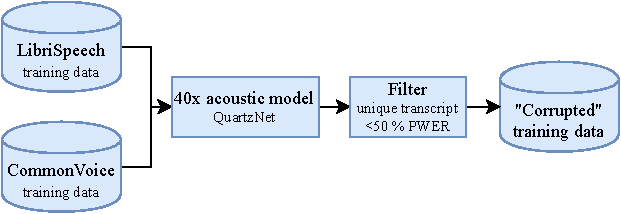
\includegraphics[width=\linewidth]{img/ensemble_diagram}
	\caption{Overview of setup for obtaining ``corrupted'' training data.}
	\label{fig:asr_folds}
\end{figure}

\subsection{Data Preparation}
To train the ensemble of the acoustic models, we use LibriSpeech and Common Voice datasets. We concatenate these two and divide them into ten folds of the same size. We deliberately not shuffle the concatenated dataset prior to splitting it into folds, so that the difference among the trained models is as much as possible (proportion of training data from LibriSpeech and from Common Voice will vary more). The models are trained on these folds in a cross-validation manner: $i$-th model skips $i$-th fold during training.

\subsection{Ensemble Training}
We train ten models. Additionally, we store checkpoints every 5000 steps. Instead of bigger Jasper, we choose QuartzNet. Nevertheless, they are similar enough, and we assume they behave likewise. The main reason for our choice are reduced hardware requirements and hence faster convergence. In contrast with the bigger ASR Jasper model that we train on 10 GPUs, each QuertzNet model for data collection is trained only on one GPU. After less than a day of training, the models perform almost as good as the bigger model.

We utilize transfer learning to reduce the training time. For English, the QuartzNet encoders are initialized with checkpoint available at NVIDIA NGC.\footnote{\url{https://ngc.nvidia.com/catalog/models/nvidia:quartznet15x5}} The model was trained on LibriSpeech and Common Voice. As the target vocabulary differs for our setup (phonemes instead of graphemes), we apply the method from chapter \ref{chapter:asr}. The training is divided into the two phases: (1) Decoder adaptation phase: the encoder is initialized with the pre-trained weights and is frozen; the decoder is randomly initialized. Only the decoder is trained. (2) Full training: the encoder is unfrozen and trained together with the decoder. The adaptation phase takes 2000 steps, and full training continues afterward for another 30000 steps.

\subsection{Acoustic Models Performance}
On average, after the first adaptation phase, the word error rate of the most models on LibriSpeech \texttt{dev-clean} dropped under 16 \% (this took approximately 5 hours). One model had WER two times worse than others (33.05 \%), and one did not converge at all. After the full training, which took about 15 hours, the average WER is 5.3 \% with very small variance. Compared with big Jasper, it is only about 1.5 \% points more. Evaluations during the training can be seen in \cref{fig:ensemble_training} and the final results are shown in \cref{tab:eng_folds}.

\begin{figure*}[t]
	\includegraphics[width=\linewidth,height=8cm]{img/ensemble}
	\caption{Evaluation on LibriSpeech \texttt{dev-clean} during the training of ten models (using greedy decoding). One epoch takes approximately 24400 steps.}
	\label{fig:ensemble_training}
\end{figure*}

\begin{table}[t]
	\centering
	\resizebox{\columnwidth}{!}{
		\begin{tabular}{l|cccccccccc}
			\bf Model & \bf 1 & \bf 2 & \bf 3 & 4 & \bf 5 & \bf 6 & \bf 7 & \bf 8 & \bf 9 & \bf 10  \\
			\hline 
			
			Adapt. phase & 15.17  & 
			15.02  & 
			16.66  & 
			22.15  & 
			15.07  & 
			15.39  & 
			15.24  & 
			17.44  & 
			15.38  & 
			33.05 \\
			Full training &
			5.07  & 
			5.21  & 
			5.16  & 
			4.99  & 
			5.22  & 
			5.34  & 
			5.45  & 
			5.31  & 
			5.30  & 
			5.98
			
		\end{tabular}
	}
	\caption{Results in \% of word error rate (using greedy decoding) on LibriSpeech \texttt{dev-clean} for all trained models.}
	\label{tab:eng_folds}
\end{table}

\subsection{English Corrupted Data Collection}
In order to generate more data, we make checkpoints during training every 5000 steps and keep the last four for every model. This gives us 40 unique models. Additionally, we employ drop-out and Cutout to gain more variability in the collected data.

Concatenated LibriSpeech and Common Voice training data are used as the source for the inference. Using all 40 models, we yield 36M sentence pairs. We keep only the pairs with unique source sentence (i.e., has a unique error) and destroy pairs with PWER over 50 \%. From the 36 million tuples, we get 7M filtered sentence pairs, particularly 3.7M from LibriSpeech and 3.3M from Common Voice.

Distribution of PWER in training and development sets is in histogram~\ref{fig:histogram}. We filter out all pairs with PWER higher than 50~\%. As we can see in the histogram~\ref{fig:histogram}, only 7~\% of all collected training data is left out. We can observe that the distribution of PWER for training data almost copy the distribution of Common Voice \texttt{dev} with training data having slightly more pairs with smaller PWER. On the other hand, LibriSpeech \texttt{dev-clean} has significantly more examples with small PWER.

\begin{table}[t]
	\centering
	\small
	\begin{tabular}{l|ccc}
		\bf Set & \bf AVG WER & \bf Median WER & \bf STD   \\
		\hline 
		Training &  10.24 \% & 2.70 \% & 16.64 \% \\
		LibriSpeech \texttt{dev-clean} &  4.33 \% & 0.0 \% & 8.37 \% \\
		Common Voice \texttt{dev} &  11.98 \% & 0.0 \% & 17.71 \% \\
	\end{tabular}
	\caption{Performance of the 40 ensemble models on the datasets.}
	\label{tab:eng_corrupted_table}
\end{table}

\begin{figure}[t]
	\includegraphics[width=\linewidth,height=8cm]{img/histogram}
	\caption{Distribution of PWER on the collected English ``corrupted'' data and the two development sets.}
	\label{fig:histogram}
\end{figure}









\section{Czech ``Corrupted'' Training Data}
\label{sec:asr_corrupted_cs}
In this section, we reproduce the previously described experiment for the Czech language. Most challenging is to overcome the scarcity of speech data. The Czech speech corpus has approximately 400h. On the other hand, the two English corpora yield together almost 2000h.

\subsection{Task Setup}
We proceed similarly to the setup described in \cref{sec:asr_corrupted}: we split the available data into ``folds''. Each fold then serves as a training corpus for one acoustic model. Unlike for the English, we decided to have only five folds instead of 10 to take the dataset size into account.

The training and collection of corrupted data remain the same.

\subsection{Ensemble Training}
Following the receipt from English, we employ QuartzNet architecture, train all models on one GPU, and follow the same transfer learning technique. We train-off from our best performing, fully trained, Czech ASR model (see \cref{chapter:asr}). Because of the Czech training data scarcity, we train only five folds. For more details regarding the training, see \cref{sec:asr_corrupted}.

\cref{fig:ensemble_training_cs} depicts the performance of the trained acoustic models on the development set during the training.

\subsection{Acoustic Models Performance}
\cref{tab:cs_folds} offers detailed training results for all models. 

We observe a dramatic PWER decline at the beginning (until step 12k), followed by almost no change until the end of the training. We assume there are two reasons for this behavior: (1) data scarcity; (2) contrast in grapheme-to-phoneme correspondence in the Czech and the English language. We assume the latter to have a more significant impact, as the model converged after 7 thousand steps, which is roughly right after seeing all examples once (2000 steps adaptation phase + one epoch of 4775 steps of the full training).

\begin{figure}[h]
	\includegraphics[width=\linewidth,height=8cm]{img/ensemble_cs}
	\caption{Evaluation of the development set during the training of the 5 models (using greedy decoding). One epoch is approximately 4750 steps.}
	\label{fig:ensemble_training_cs}
\end{figure}

\begin{table}[h]
	\centering
	\begin{tabular}{l|cccccccccc}
		\bf Model & \bf 1 & \bf 2 & \bf 3 & 4 & \bf 5  \\
		\hline 
		
		Adapt. phase &
		97.91 &
		17.63 &
		13.53 &
		14.09 &
		13.37 \\
		Full training &
		7.17 &
		7.03 &
		7.14 &
		7.25 &
		7.13 
		
	\end{tabular}
	\caption{Results in \% of PWER (greedy decoding) on the development set for all trained models.}
	\label{tab:cs_folds}
\end{table}

\subsection{Czech Corrupted Data Collection}
In order to generate more data, we make checkpoints during training every 5000 steps and keep the last four for every model. This gives us 20 unique models. Additionally, we employ drop-out and Cutout to gain more variability in the collected data.

We use the training data of the Czech Parliament Hearings dataset as the source for the inference. Using all 20 models, we yield 3.8M sentence pairs. This is almost ten times less than for English. We keep only the pairs with unique source sentences (i.e., has a unique error) and destroy pairs with PWER over 50 \%. Finally, we get two million sentence pairs.

Distribution of PWER in training and dev sets is in histogram~\ref{fig:histogram}. We filter out all pairs with PWER greater than 50~\%. As we can see in the histogram~\ref{fig:histogram}, only 13~\% of all collected training data is removed. We can observe that the collected data contains more recordings with higher PWER than the test set. 

\begin{figure}[t]
	\includegraphics[width=\linewidth,height=8cm]{img/histogram_cs}
	\caption{Distribution of PWER of the collected Czech ``corrupted'' data and the Czech Parliament Hearings test set. Note, we used the test set instead of the development set. PWER of the recordings in the development set does not correspond to the actual sentence-level distribution of PWER. This is because the development set contains 12  further unsegmented recordings each more than 10 minutes long.}
	\label{fig:histogram_cs}
\end{figure}

\section{Fine-Tuning of Enhanced ASR}















\iffalse 
\begin{figure}[h]
	\centering
	\begin{tikzpicture}[thick, node distance=2.5cm, 
	>=stealth,
	bend angle=45,
	auto,regentonne/.style={cylinder,aspect=0.3,draw,shape border rotate=90}]
	\draw
	node at (0,0)[block,regentonne] (libri) {\shortstack{LibriSpeech\\ \small{training data}}}
	node [block, below right=0.4cm of libri] (ensemble1) {\shortstack{$40 \times$ QuartzNet\\ \small{small models}}}
	node [block,regentonne, below =1.5cm of libri] (common) {\shortstack{Common Voice\\ \small{training data}}}
	
	node at (0,-6) [block,regentonne] (libri_dev) {\shortstack{LibriSpeech\\ \small{dev}}}
	node [block,regentonne, below =0.3cm of libri_dev] (common_dev) {\shortstack{Common Voice\\ \small{dev}}}
	
	node at (5,-7) [block] (jasper) {\shortstack{Jasper\\ \small{big model} \\ \small{from final pipeline}}}
	
	node [block, right=1cm of ensemble1] (filter) {\shortstack{filter\\ \small unique source\\ $<$50\% WER}}
	
	node [block,regentonne,right=1cm of filter] (training) {\shortstack{``corrupted''\\ training data}}
	
	node at (10,-6) [block,regentonne] (libri_dev2) {\shortstack{``corrupted''\\LibriSpeech\\ \small{dev}}}
	node [block,regentonne, below =0.3cm of libri_dev2] (common_dev2) {\shortstack{``corrupted''\\Common Voice\\ \small{dev}}};
	
	\draw[->](libri) -> node {}  (ensemble1);
	\draw[->](common) -> node  {} (ensemble1);
	\draw[->](ensemble1) -> node {}  (filter);
	\draw[->](filter) -> node {}  (training);
	\draw[->](libri_dev) -> node {}  (jasper);
	\draw[->](common_dev) -> node {}  (jasper);
	\draw[->](jasper) -> node {}  (libri_dev2);
	\draw[->](jasper) -> node {}  (common_dev2);
	
	\end{tikzpicture}
	\caption{After training of 10 ``smaller'' QuartzNet models with 4 chechpoints made along the way (hence $40 \times$), training data are transcribed and filtered. Similarly, Development sets are transcribed using ``bigger'' Jasper model that will be in the final ASR pipeline (see \cref{fig:asr_enhanced_pipeline}).}
	\label{fig:asr_folds_}
\end{figure} 
\fi